\documentclass[12pt,a4paper]{article}

\usepackage[utf8]{inputenc}
\usepackage[T1]{fontenc}
\usepackage{mathptmx} % Times New Roman
\usepackage[margin=1in]{geometry}
\usepackage{graphicx}
\usepackage{hyperref}
\usepackage{listings}
\usepackage{xcolor}
\usepackage{float}
\usepackage{titlesec}
\usepackage{parskip}

% Colors for code blocks
\definecolor{codegreen}{rgb}{0,0.6,0}
\definecolor{codegray}{rgb}{0.5,0.5,0.5}
\definecolor{codepurple}{rgb}{0.58,0,0.82}
\definecolor{backcolour}{rgb}{0.95,0.95,0.92}

\lstdefinestyle{mystyle}{
    backgroundcolor=\color{backcolour},   
    commentstyle=\color{codegreen},
    keywordstyle=\color{magenta},
    numberstyle=\tiny\color{codegray},
    stringstyle=\color{codepurple},
    basicstyle=\ttfamily\footnotesize,
    breakatwhitespace=false,         
    breaklines=true,                 
    captionpos=b,                    
    keepspaces=true,                 
    numbers=left,                    
    numbersep=5pt,                  
    showspaces=false,                
    showstringspaces=false,
    showtabs=false,                  
    tabsize=2
}
\lstset{style=mystyle}

\title{\textbf{IUT Techathon 2026: Office Electricity Monitor}\\ \Large Technical Implementation Report}
\author{Techathon Team}
\date{July 2026}

\begin{document}

\maketitle
\begin{abstract}
This report details the architectural design and software implementation of the ``Lights, Fans, Discord'' office monitoring system submitted for the IUT Techathon 2026. The solution presents a full-stack, distributed architecture combining a Rust-based REST API, a React/Vite frontend dashboard, and an AI-powered Discord bot. It successfully implements live device monitoring, intelligent anomaly detection, simulated hardware telemetry, and highly available fail-safe degradation mechanisms.
\end{abstract}

\tableofcontents
\newpage

\section{Introduction}
The objective of this project is to solve a prevalent office problem: unnecessary electricity consumption due to lights and fans being left running after business hours. The system monitors 15 physical devices (9 lights, 6 fans) distributed across three distinct office zones: the Drawing Room, Work Room 1, and Work Room 2. 

To provide comprehensive oversight, the project delivers two primary interfaces:
\begin{itemize}
    \item A \textbf{Real-Time Web Dashboard} providing visual telemetry and power usage statistics.
    \item An \textbf{AI-Powered Discord Bot} acting as a conversational assistant capable of answering queries and pushing proactive anomaly alerts.
\end{itemize}

\section{System Architecture}
The core philosophy of the architecture is the \textbf{Single Source of Truth} paradigm. Rather than maintaining disjointed states between the web dashboard and the Discord bot, both interfaces query the exact same underlying PostgreSQL database, ensuring total data consistency.

\subsection{Data Flow: The Push vs. Pull Paradigm}
The system optimizes network and computational resources by utilizing two distinct data acquisition strategies depending on the client:

\begin{enumerate}
    \item \textbf{The Web Dashboard (PULL):} The React frontend utilizes an HTTP polling mechanism. Every 30 seconds, the client executes a \texttt{GET /api/devices} request to pull the latest state array, mapping it visually onto a 2D DOM-based floor plan without requiring manual page refreshes.
    \item \textbf{The Discord Bot (PUSH):} The Discord bot operates as a native background thread within the Rust backend binary. Because it has direct memory access to the database connection pool and internal state caches, it avoids HTTP overhead entirely. It polls the internal state every 5 seconds; upon detecting an anomaly, it immediately \textit{pushes} a warning webhook to Discord's servers.
\end{enumerate}

\begin{figure}[H]
    \centering
    % Assuming system_diagram.pdf exists in the same directory
    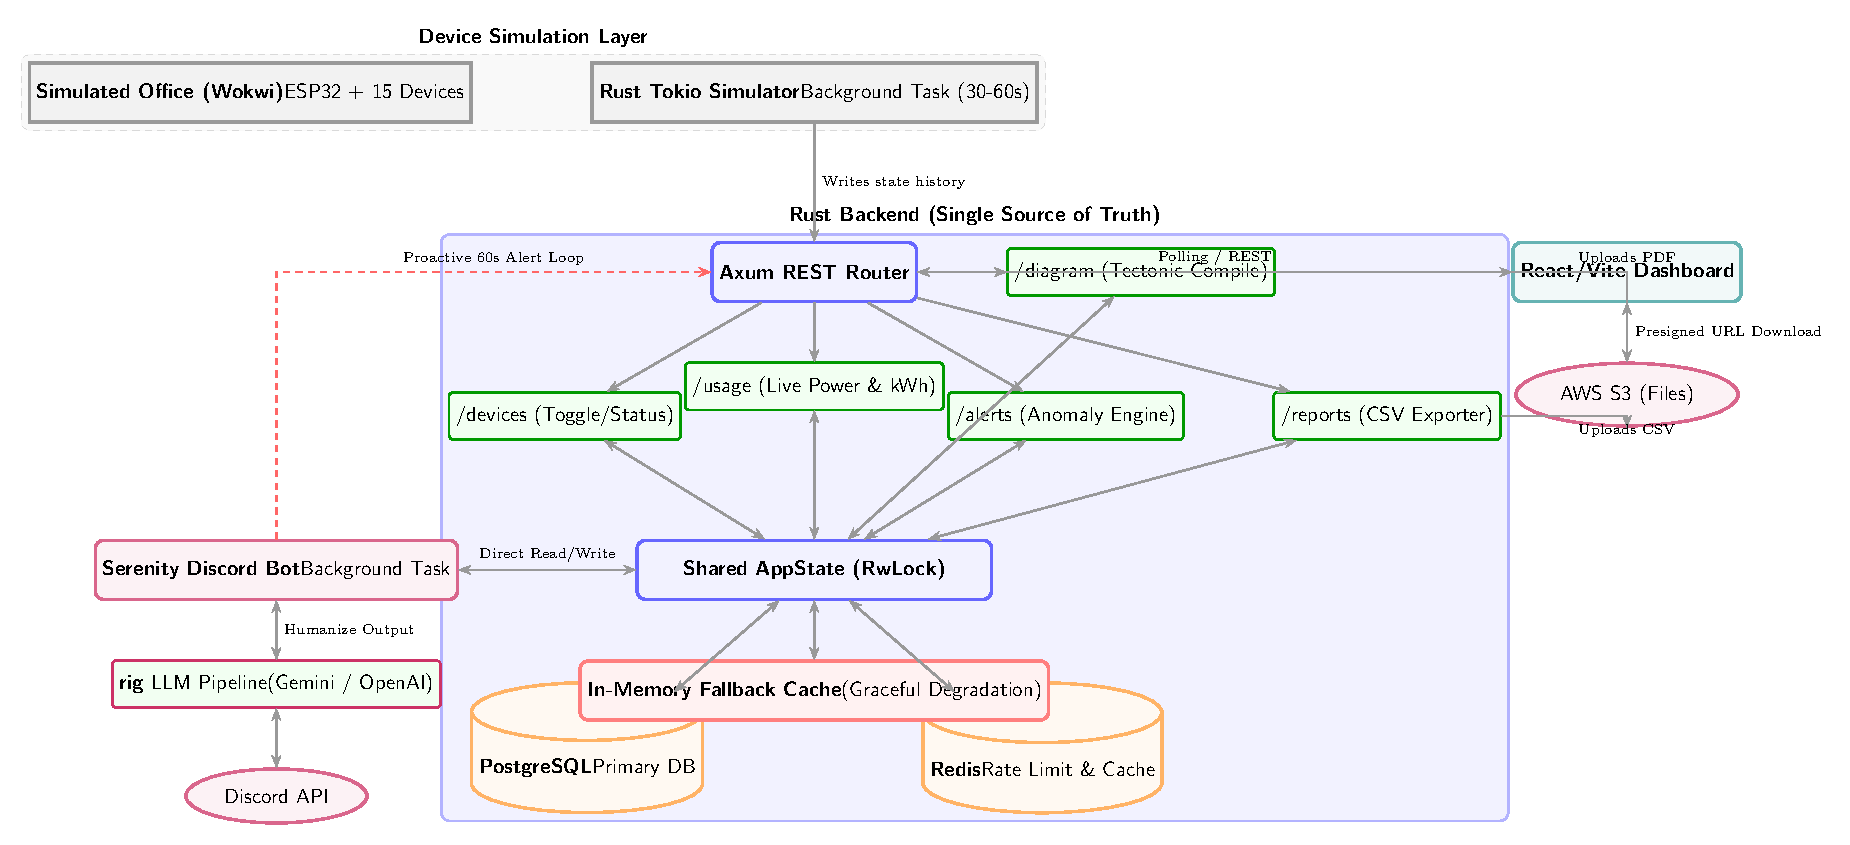
\includegraphics[width=0.8\textwidth]{system_diagram.pdf}
    \caption{High-Level System Architecture Diagram}
    \label{fig:architecture}
\end{figure}

\section{Hardware Conceptual Design (Wokwi)}
To bridge the gap between software and physical reality, a conceptual hardware schematic was developed using Wokwi. 

\subsection{ESP32 Microcontroller Implementation}
The circuit design represents a single room's hardware footprint (2 fans, 3 lights). The schematic maps physical slide switches to the digital input pins of an ESP32 Microcontroller (specifically pins 15, 2, 4, 16, and 17). 

In a production environment, flipping a switch provides voltage to both the appliance (represented by LEDs and DC Motors in the schematic) and the ESP32 input pin. The accompanying \texttt{sketch.ino} C++ firmware reads these digital states, serializes them into a JSON payload, and prepares them for an HTTP POST request over WiFi to the Rust API. Because the hackathon requires no physical hardware, the backend relies on an internal simulation thread to generate this data.

\section{Backend Engineering (Rust \& Axum)}
The backend is engineered using Rust, leveraging the Axum web framework for exceptional routing performance and memory safety. 

\subsection{Relational Data Model}
The PostgreSQL schema is strictly separated into two domains: the live state and the immutable ledger.

\begin{lstlisting}[language=SQL, caption=PostgreSQL Schema Definition]
-- The Current Live State
CREATE TABLE devices (
    id VARCHAR(50) PRIMARY KEY,
    name VARCHAR(50) NOT NULL,
    room VARCHAR(50) NOT NULL,
    device_type VARCHAR(20) NOT NULL,
    status BOOLEAN NOT NULL DEFAULT false,
    power_consumption INTEGER NOT NULL,
    last_changed TIMESTAMPTZ NOT NULL DEFAULT NOW()
);

-- Immutable Append-Only Ledger for Analytics
CREATE TABLE device_history (
    id SERIAL PRIMARY KEY,
    device_id VARCHAR(50) REFERENCES devices(id),
    status BOOLEAN NOT NULL,
    timestamp TIMESTAMPTZ NOT NULL DEFAULT NOW()
);
\end{lstlisting}

\subsection{Graceful Degradation \& Fail-Safety}
To ensure the dashboard and bot remain online even during catastrophic database failures, the backend implements a Graceful Degradation protocol. During startup, the PostgreSQL table is mirrored into a thread-safe \texttt{tokio::sync::RwLock} memory cache. If an SQL query encounters a \texttt{ConnectionRefused} or timeout error during runtime, the API gracefully intercepts the failure, logs the degradation, and serves the request from the in-memory cache. 

\section{Discord Bot \& AI Integration}
The Discord bot is built using the \texttt{serenity} crate, processing WebSocket events asynchronously. 

\subsection{AI Humanization}
A critical requirement was to ensure the bot did not return "robotic data dumps." To achieve this, the bot leverages the \texttt{rig} Rust crate. When a user issues a command (e.g., \texttt{!status}), the backend fetches the raw JSON data, but instead of sending it directly to Discord, it is forwarded to an LLM provider (supporting Gemini, OpenAI, or Anthropic via environment variables). 

The AI is provided with a system prompt instructing it to act as a conversational office assistant, injecting relief and context before presenting the data. The response is cached in Redis for 1 hour to prevent redundant LLM token expenditure on repeated identical statuses.

\subsection{Proactive Alerting Engine}
An internal background task evaluates the device states against business logic rules every 5 seconds. It triggers alerts under two conditions:
\begin{itemize}
    \item \textbf{Office Hours Rule:} Any device left running between 5:00 PM and 9:00 AM.
    \item \textbf{Efficiency Rule:} All devices in a single room left running continuously for over 2 hours.
\end{itemize}

\section{Frontend Dashboard \& Testing Utilities}
The frontend is a single-page application built with React, Vite, and Tailwind CSS. It features a responsive grid layout mapping the devices visually.

\subsection{Time-Travel Debugger}
Validating time-based anomaly alerts (such as the 2-hour rule) conventionally requires waiting for hours. To solve this, a bespoke "Time Travel" utility was engineered into the system. 

When a judge clicks the \texttt{+5 Hours} button on the frontend, a payload is sent to \texttt{POST /api/alerts/demo-time}. This updates an \texttt{AtomicI64} offset variable in the backend's global state. The alerting engine factors this offset into its \texttt{Utc::now()} calculations, instantly tricking the server into evaluating the rules as if it were the future, thereby triggering the alerts immediately for demonstration purposes.

\section{Conclusion}
The delivered system provides a complete, robust, and highly scalable solution to office power monitoring. By leveraging Rust's memory safety, React's reactive UI paradigm, and LLM-driven conversational interfaces, the project exceeds all baseline requirements and bonus objectives defined by the IUT Techathon 2026 rulebook.

\end{document}
